%!TEX root = ../report.tex

\begin{figure}
	\centering
	\captionsetup{font=small}
    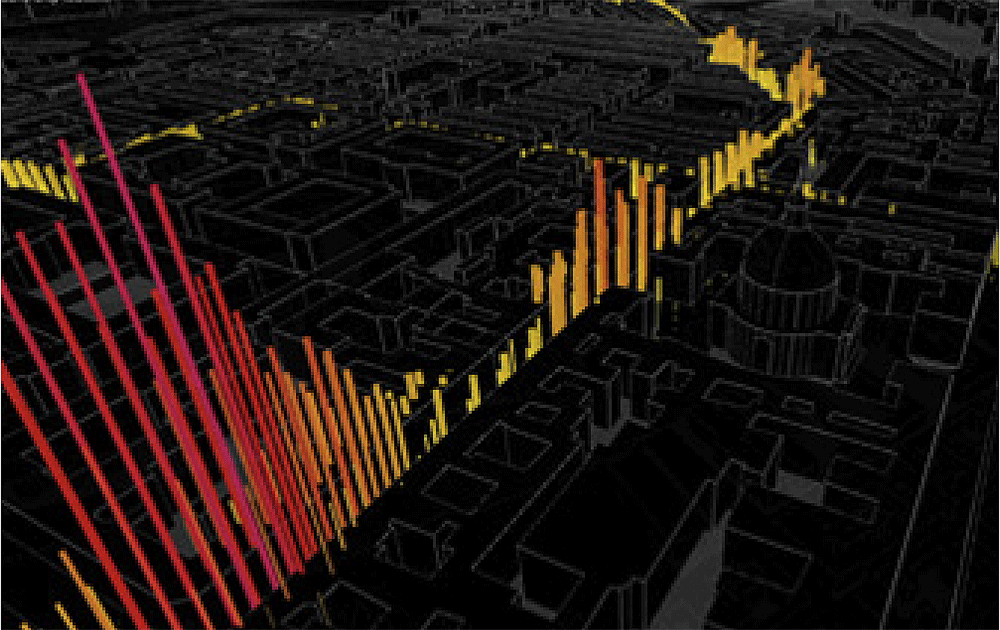
\includegraphics[width=0.8\textwidth]{images/literature/category-combination}
	\caption[Abstract geovisualisation technique]{An example of combining 3D representations of the real world with abstract data. \protect\footnotemark}
	\label{fig:category_combination}
\end{figure}

\footnotetext{\bibentry{ratti2010copenhagen}}
